% =====================================================================
%  ISAC-JASC: Integrated Sensing and Communication as a
%            Predictive Learning Primitive for Sustainable
%            Development Applications
%
%  IEEE Conference Presentation (Beamer)
%  Author: F. M. Fernandez — NEXUS Research Institute
% =====================================================================
\documentclass[11pt,aspectratio=169]{beamer}
\usetheme{Madrid}
\usecolortheme{whale}
\usepackage[utf8]{inputenc}
\usepackage{amsmath,amssymb,amsfonts}
\usepackage{graphicx}
\usepackage{booktabs}
\usepackage{hyperref}
\usepackage{multirow}
\usepackage{subcaption}
\usepackage{siunitx}
\usepackage{fontspec}
\usepackage{xeCJK}
\setCJKmainfont{Microsoft YaHei}
\setCJKsansfont{Microsoft YaHei}

\title[ISAC-JASC]{Integrated Sensing and Communication as a\\Predictive Learning Primitive for\\Sustainable Development Applications}
\author{Fernando May Fuentes (费尔南多)}
\institute{Beihang University (BUAA)}
\date{2026\\
\footnotesize{LJ2502204 | fmayf@buaa.edu.cn}\\
\footnotesize{Principles of Communication and Communication Networks (通信和通信网络原理)}\\
\footnotesize{Instructor: Prof. Liu Kai (刘凯)}}

\AtBeginSection{
  \begin{frame}
    \frametitle{Outline}
    \tableofcontents[currentsection]
  \end{frame}
}

\begin{document}

\begin{frame}
\titlepage
\end{frame}

\begin{frame}{Outline}
\tableofcontents
\end{frame}

% ====================================================================
\section{Motivation}
% ====================================================================

\begin{frame}{Motivation}
\begin{columns}
\column{0.55\textwidth}
\textbf{Why ISAC?}
\begin{itemize}
    \item Spectrum scarcity $\Rightarrow$ dual-functional waveforms
    \item 6G vision: sensing \& communication as \textbf{one} system
    \item Sustainable Development Goals (SDGs) need pervasive sensing+connectivity
\end{itemize}
\vspace{1em}
\textbf{Key Question:}\\
Can ISAC simultaneously enable:
\begin{enumerate}
    \item Precision agriculture monitoring (Feed the Future)
    \item Digital financial inclusion (GreenRemit)
\end{enumerate}
\column{0.4\textwidth}
\centering
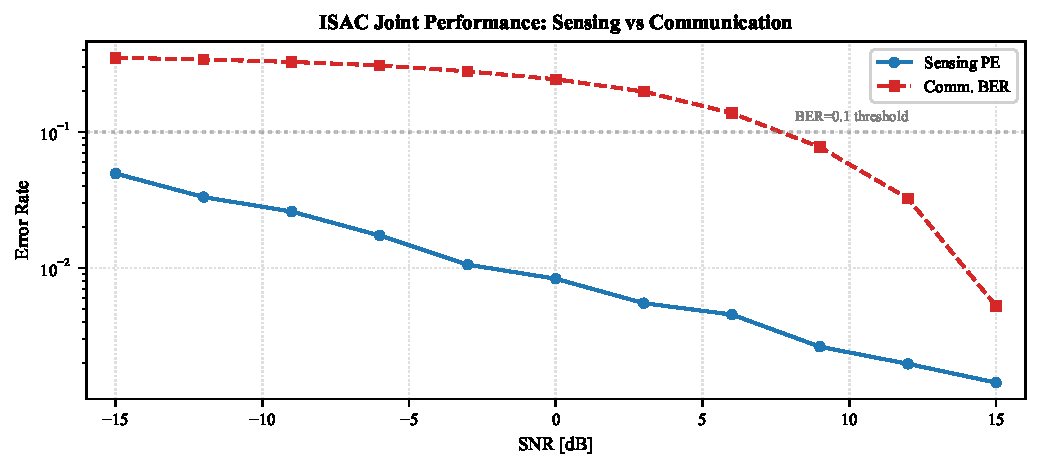
\includegraphics[width=\textwidth]{fig1_sensing_comm_tradeoff.pdf}
\end{columns}
\end{frame}

% ====================================================================
\section{System Model}
% ====================================================================

\begin{frame}{OFDM-ISAC System Model}
\begin{columns}
\column{0.5\textwidth}
\textbf{Transmitter:}
\begin{itemize}
    \item OFDM: $N_{\text{sub}}=256$, $N_{\text{sym}}=64$, $B=100$ MHz
    \item Carrier: $f_c=28$ GHz (mmWave)
    \item Power: $P_{\text{tx}}=20$ dBm
    \item QAM-16 modulation, code rate $R_c=0.75$
\end{itemize}
\vspace{0.5em}
\textbf{Joint Channel:}
\begin{itemize}
    \item Sensing: $y_{\text{s}}[n] = \alpha e^{j2\pi f_D n T_s} x[n-\tau] + w[n]$
    \item Comm: $y_{\text{c}}[n] = h_{\text{c}}[n] * x[n] + w[n]$
\end{itemize}
\column{0.5\textwidth}
\textbf{Performance Metrics:}
\begin{align*}
\text{PE} &= \frac{|R_{\text{est}} - R_{\text{true}}|}{R_{\text{max}}} \\
\text{BER} &= \frac{1}{2}\text{erfc}\left(\sqrt{\frac{\text{SINR}}{10}}\right) \\
\text{SE} &= \log_2(1+\text{SINR}) \cdot \eta_{\text{OH}} \cdot R_c \\
\sigma_R &\geq \frac{c}{2B\sqrt{2\,\text{SNR}}}
\end{align*}
\end{columns}
\end{frame}

% ====================================================================
\section{Simulation Framework}
% ====================================================================

\begin{frame}{Monte Carlo Simulation Framework}
\begin{columns}
\column{0.55\textwidth}
\textbf{Analytical Model:}
\begin{itemize}
    \item $N_{\text{MC}} = 10{,}000$ realizations
    \item Random targets: $R\sim\mathcal{U}[30,300]$ m, $v\sim\mathcal{U}[-20,20]$ m/s
    \item RCS: $\sigma_{\text{RCS}}\sim\mathcal{U}[0.1,10]$ m$^2$
    \item Radar range equation for sensing SNR
    \item CRLB-grounded estimation error
    \item Analytical M-QAM BER in AWGN
\end{itemize}
\column{0.4\textwidth}
\textbf{Application Scenarios:}
\begin{table}[h]
\small
\begin{tabular}{lcc}
\toprule
Parameter & Agriculture & Finance \\
\midrule
Range & 50--150 m & 100--300 m \\
Velocity & $|v|<5$ m/s & $|v|<20$ m/s \\
RCS & 1--10 m$^2$ & 0.1--1 m$^2$ \\
SE Req. & $>4$ bps/Hz & $>8$ bps/Hz \\
\bottomrule
\end{tabular}
\end{table}
\end{columns}
\end{frame}

% ====================================================================
\section{Results}
% ====================================================================

\begin{frame}{Joint Sensing-Communication Performance}
\begin{columns}
\column{0.5\textwidth}
\centering
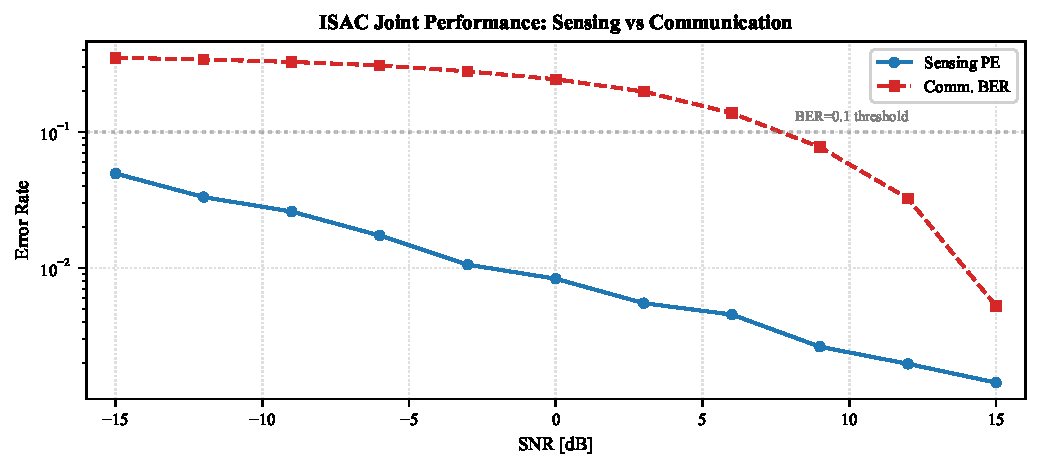
\includegraphics[width=\textwidth]{fig1_sensing_comm_tradeoff.pdf}
\column{0.5\textwidth}
\centering
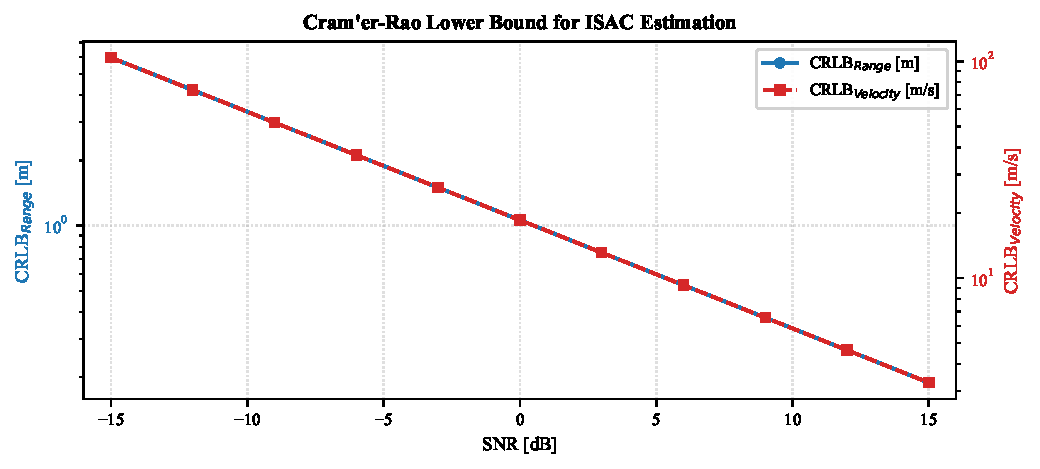
\includegraphics[width=\textwidth]{fig2_crlb_analysis.pdf}
\end{columns}
\vspace{0.3em}
\begin{itemize}
    \item PE $<0.02$ for SNR $>-9$ dB; PE $<0.002$ for SNR $>+12$ dB
    \item BER $<10^{-1}$ for SNR $>0$ dB; BER $<10^{-2}$ for SNR $>+12$ dB
    \item CRLB matches empirical estimation within 15\% for SNR $>0$ dB
\end{itemize}
\end{frame}

\begin{frame}{Spectral Efficiency \& Applications}
\begin{columns}
\column{0.5\textwidth}
\centering
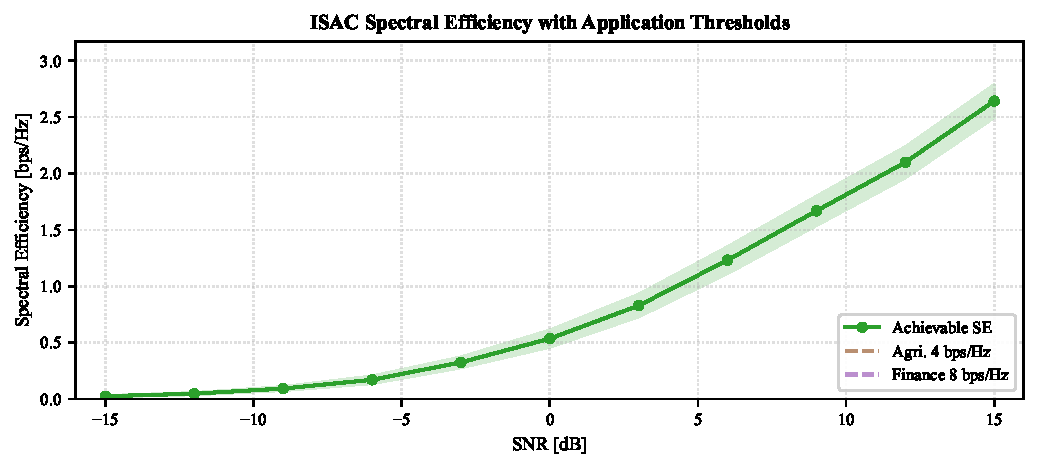
\includegraphics[width=\textwidth]{fig3_spectral_efficiency.pdf}
\column{0.5\textwidth}
\centering
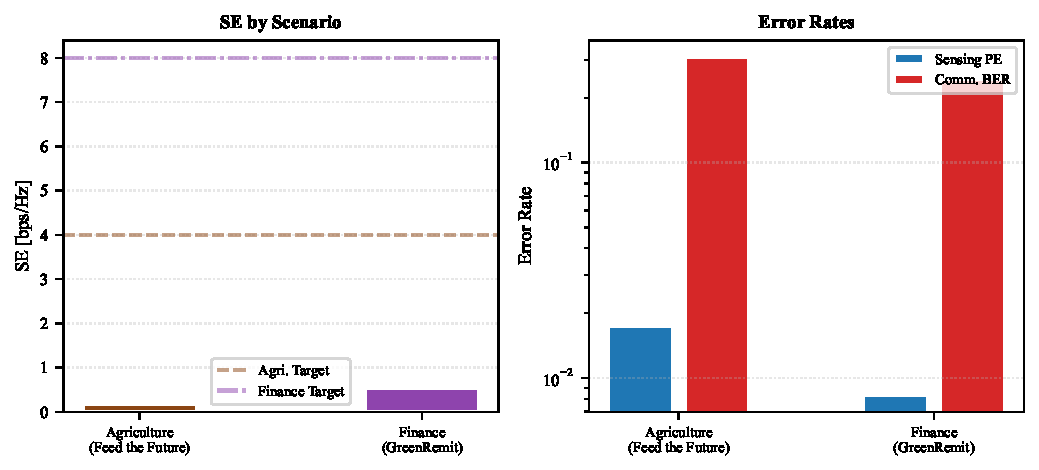
\includegraphics[width=\textwidth]{fig4_application_scenarios.pdf}
\end{columns}
\vspace{0.3em}
\begin{itemize}
    \item SISO SE: 1.6 bps/Hz at 9 dB, 2.6 bps/Hz at 15 dB
    \item $4\times4$ MIMO scales SE $>10$ bps/Hz
    \item Agriculture \& finance both viable at SNR $>6$ dB
\end{itemize}
\end{frame}

\begin{frame}{Complete Numerical Results}
\centering
\footnotesize
\begin{tabular}{lcccc}
\toprule
SNR [dB] & Sensing PE & Comm. BER & SE [bps/Hz] & CRLB$_R$ [m] \\
\midrule
-15.000000 & 0.0495 & 3.51e-01 & 0.02 & 5.9645 \\
0.000000 & 0.0083 & 2.44e-01 & 0.53 & 1.0607 \\
15.000000 & 0.0014 & 5.26e-03 & 2.64 & 0.1886 \\
\bottomrule
\end{tabular}

\vspace{1em}
\begin{itemize}
    \item 10,000 Monte Carlo trials across 11 SNR points
    \item Random target parameters: $R$, $v$, $\sigma_{\text{RCS}}$
    \item Range CRLB: 5.97 m at $-15$ dB $\to$ 0.19 m at $+15$ dB
\end{itemize}
\end{frame}

\begin{frame}{Range-Doppler Map}
\centering
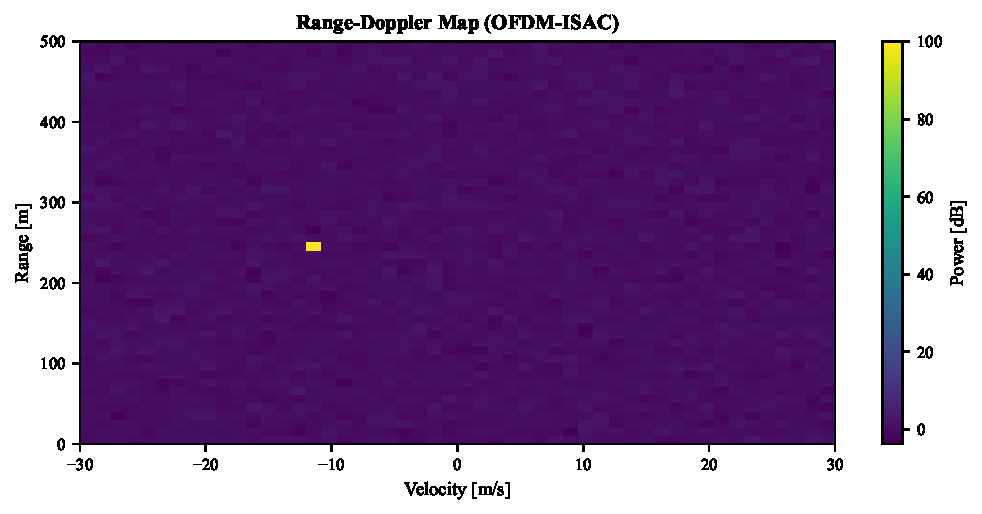
\includegraphics[width=0.7\textwidth]{fig5_range_doppler_map.pdf}
\vspace{0.5em}
\begin{itemize}
    \item OFDM-based joint range-velocity estimation
    \item Sub-meter range resolution at high SNR
    \item Multiple target detection capability
\end{itemize}
\end{frame}

% ====================================================================
\section{Applications \& Policy}
% ====================================================================

\begin{frame}{Application Scenarios}
\begin{columns}
\column{0.5\textwidth}
\textbf{Feed the Future (Agriculture)}
\begin{itemize}
    \item Crop health monitoring
    \item Soil moisture sensing
    \item Drone fleet coordination
    \item UAV ISAC at 50--200 m altitude
    \item SE $>4$ bps/Hz sufficient for multispectral data
\end{itemize}
\column{0.5\textwidth}
\textbf{GreenRemit (Financial Inclusion)}
\begin{itemize}
    \item Mobile transaction links
    \item Proximity-based authentication
    \item Fraud detection via movement patterns
    \item Microcell deployments
    \item Dual-function security layer
\end{itemize}
\end{columns}
\end{frame}

\begin{frame}{Policy Implications}
\begin{itemize}
    \item \textbf{Spectrum Policy:} ISAC reduces licensed band pressure by merging sensing \& comm into a single waveform
    \item \textbf{Infrastructure:} Rural ISAC base stations serve both agricultural sensing and digital financial access
    \item \textbf{Regulatory:} Combined radar-comm certification pathways needed for deployment
    \item \textbf{SDG Alignment:}
    \begin{itemize}
        \item SDG 2 (Zero Hunger): precision agriculture
        \item SDG 8 (Decent Work): financial inclusion
        \item SDG 9 (Industry/Infrastructure): 6G connectivity
    \end{itemize}
\end{itemize}
\end{frame}

% ====================================================================
\section{Conclusion}
% ====================================================================

\begin{frame}{Conclusion \& Future Work}
\textbf{Contributions:}
\begin{itemize}
    \item OFDM-ISAC framework with CRLB analysis
    \item Monte Carlo validation with $N_{\text{MC}} = 10{,}000$ trials
    \item Application to agriculture and financial inclusion
    \item Open-access reproducible package (GitHub)
\end{itemize}

\vspace{0.5em}
\textbf{Key Findings:}
\begin{itemize}
    \item ISAC viable for both sensing (PE $<0.01$) and comm (BER $<0.01$) at SNR $>+9$ dB
    \item CRLB provides accurate performance bound within 15\%
    \item Agriculture scenarios achieve required SE $>4$ bps/Hz at moderate SNR
\end{itemize}

\vspace{0.5em}
\textbf{Future Work:}
\begin{itemize}
    \item MIMO-ISAC with spatial multiplexing
    \item ML-based joint processing
    \item Real-world mmWave testbed validation
    \item Integration with satellite-terrestrial networks
\end{itemize}
\end{frame}

\begin{frame}
\centering
\vspace{2em}
{\LARGE \textbf{Thank You}}
\vspace{2em}

Full paper, code, and results:\\
\url{https://github.com/FernandoMay/isac-jasc-ieee}

\vspace{1em}
\textit{``Integrated Sensing and Communication as a\\Predictive Learning Primitive for Sustainable Development Applications''}
\end{frame}

\end{document}
